\documentclass[tikz, border=10pt]{standalone}

\usepackage{verbatim}

\begin{comment}
:Title: MESIF protocol
:Tags: Diagrams;Block diagrams;Computer science
:Author: Marek Fiser
:Slug: mesif

A diagram describing the MESIF protocol: http://en.wikipedia.org/wiki/MESIF_protocol
\end{comment}
\usetikzlibrary{arrows}
\begin{document}

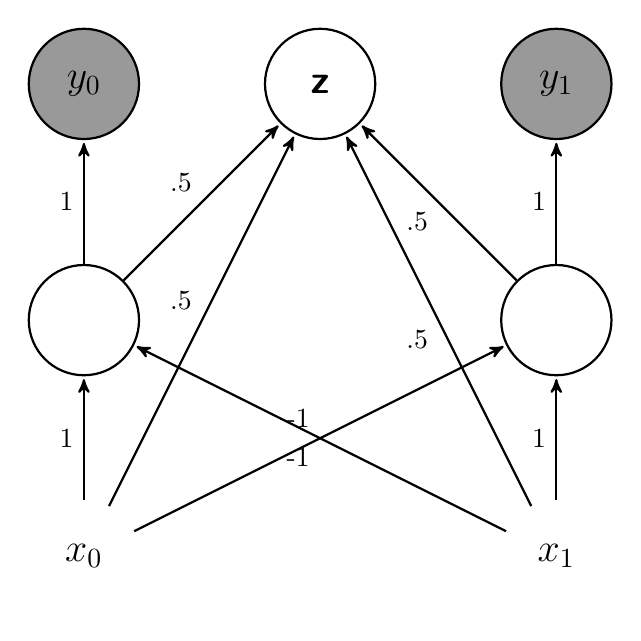
\begin{tikzpicture}[->,>=stealth',shorten >=1pt,auto,node distance=3cm,line width=4pt,
  thick,main node/.style={circle,fill=black!40,draw,
  font=\sffamily\Large\bfseries,minimum size=14mm}]
\node[main node](A){$y_0$};
 \node[main node] (Z) [right of=A,fill=white!20] {z};
 \node[main node] (B) [right of=Z] {$y_1$};
\node[main node](C)[below of=A,fill=white!20]{};
\node[main node](D)[below of=B,fill=white!20]{};
\node[main node,draw=white](E)[below of=C,fill=white!20]{$x_0$};
\node[main node,draw=white](F)[below of=D,fill=white!20]{$x_1$};
\path[every node/.style={font=\sffamily\small,
  		fill=black,inner sep=1pt}];
\path (F) edge node {.5} (Z);
\path (F) edge node {1}( D);
\path (F) edge node {-1} (C);
\path (D) edge   node {1} (B);
\path (E) edge  node {-1} (D);
\path (E) edge  node {.5} (Z);
\path (E) edge   node {1}(C);
\path (C) edge  node {1} (A);
\path (C) edge   node {.5}(Z);
\path (D) edge  node {.5} (Z);

 
\end{tikzpicture}
\end{document}
